\section{Middle-Phase Thrashing in Agentic Batch Inference}
\label{sec:motivation}



Agentic batch inference exhibits system behaviors that fundamentally differ from conventional batched LLM serving.
In this section, we uncover and characterize \textit{middle-phase thrashing}, induced by asynchronous agent progress under limited GPU memory, and show how it leads to catastrophic throughput collapse at high concurrency.
We first illustrate the root cause via a simplified workflow example, and then validate the phenomenon using empirical measurements from real-world deployments.

\subsection{Agent-Level Asynchrony and KV Cache Contention}
% Unlike standard inference workloads, where each request executes a single, contiguous generation pass, agentic inference consists of long-lived agents that repeatedly alternate between generation and external tool execution.
% Each agent accumulates context incrementally, causing its KV cache footprint to grow monotonically over time.
% Critically, agents progress through these steps asynchronously: some agents may be actively making generation requests, while others are paused waiting for tool responses.
% Figure \ref{fig:kv_overview} (a) illustrates a simplified execution workflow involving two agents, Agent 1 and Agent 2, sharing a finite number of GPU-resident KV cache slots.
% At early execution steps, both agents maintain small KV footprints, and their combined working set fits comfortably within GPU memory.
% During this phase, KV cache hit rates remain high, and batching efficiency is preserved.
% As execution proceeds, both agents accumulate longer contexts.
% When one agent enters a tool-calling phase, its KV cache becomes temporarily inactive.
% Under standard LRU-based cache management, this inactive state causes its KV entries to lose recency and become eviction candidates.
% When the second agent continues generating and expands its KV footprint, the system may evict the paused agent’s cache to satisfy immediate memory demand.
% When the paused agent later resumes generation, its KV cache is no longer resident.
% The serving engine must therefore reconstruct the entire prefix via prefill recomputation or CPU-to-GPU cache reload, incurring substantial latency and compute overhead.
% This recomputation is not attributable to model complexity or token length, but rather to inter-agent interference caused by asynchronous execution and limited cache capacity.
% Importantly, this behavior emerges even when the total number of agents is fixed.
% It is the misalignment in agent progress, rather than sheer concurrency alone, that triggers cache eviction and recomputation cascades.

Figure \ref{fig:twoagent}a
illustrates two agents sharing a finite pool of GPU-resident KV cache slots. When Agents 1 \& 2 (A1 and A2) pause for tool execution, their KV cache slots become inactive.  Under the standard LRU eviction policy, these entries lose recency and become prime candidates for eviction as Agent 3 (A3) continues to generate and consume memory. 
Consequently, when the paused agents (A1 and A2) resume, the serving engine must reconstruct the entire prefix via prefill recomputation, incurring significant latency. This example captures only the simplest case of contention between two agents.
When many agents coexist in the system, such mutual eviction and recomputation events occur far more frequently, as agents repeatedly alternate between active generation and tool-induced pauses.
These cascading evictions lead to persistent cache churn during the middle stages of agent execution, ultimately giving rise to the \emph{middle-phase thrashing} phenomenon, which we formally characterize below.
% in \S\ref{subsec:character-middle-phase}.



% Due to the inherent nature of multi-turn agent tool use, it is anticipated that current prefixes will be frequently reused. Rather than resorting to offloading or eviction, this characteristic provides an opportunity to strategically reject certain requests in anticipation of imminent, identical agent queries that can leverage the existing KV cache.


% This overhead stems not from model complexity or token length, but from middle-phase thrashing: a misalignment in progress that triggers eviction cascades even when the number of agents remains fixed.

% % \subsection{Three-Phase Evolution of KV Cache Pressure}
% \subsection{Middle-Phase Thrashing of serving engines}
% % When many agents execute concurrently, the above interaction generalizes into a characteristic three-phase execution pattern in terms of aggregate KV cache usage and cache efficiency.
% % Warmup Phase.
% % At the beginning of execution, most agents operate at early reasoning steps with short contexts.
% % KV cache footprints are small and highly similar, often benefiting from prefix sharing.
% % During this phase, increasing concurrency improves throughput, KV cache hit rates remain high, and GPU utilization scales favorably.
% % Oscillation Phase.
% % As agents advance into mid-horizon steps, their contexts diverge and lengthen.
% % Prefix sharing diminishes, and the aggregate KV cache demand grows rapidly.
% % Since agents progress asynchronously, frequently pausing for tool calls and resuming generation, the active working set fluctuates over time.
% % Under fixed GPU memory capacity, this leads to aggressive cache eviction and reload cycles.
% % The system enters a thrashing regime, where KV cache usage remains near saturation while KV cache hit rates collapse.
% % In this phase, additional concurrency paradoxically reduces overall throughput due to excessive recomputation and scheduling fragmentation.
% % Cooldown Phase.
% % Eventually, a subset of agents completes execution and releases their KV cache state.
% % As memory pressure subsides, eviction frequency decreases and cache hit rates partially recover.
% % Throughput improves relative to the oscillation phase, though it typically does not return to warmup-level efficiency due to residual fragmentation.
% % This phase-dependent behavior explains why offline agentic inference exhibits a non-monotonic relationship between concurrency and throughput, in contrast to traditional LLM inference where throughput degrades only upon outright memory exhaustion.

% When scaling the concurrency of agents, the interference mechanism described above generalizes into a characteristic three-phase pattern regarding aggregate KV cache usage and efficiency.

% \noindent\textbf{Warmup Phase}. 
% During the initial execution stage, agents operate at shallow reasoning depths with limited context lengths and shared prefixes of prompts. Consequently, KV cache footprints remain small and exhibit high similarity, enabling the serving engine to maximize prefix sharing. 
% In this phase, increasing concurrency yields monotonic throughput gains; KV cache hit rates approach 100\%, and GPU utilization scales efficiently as the aggregate working set remains well within memory constraints.

% \noindent\textbf{Middle Phase}. 
% As agents advance into mid-horizon steps, their contexts diverge and lengthen, diminishing opportunities for prefix sharing while rapidly increasing aggregate memory demand. 
% Since agents progress asynchronously and may encounter frequent pausing and resuming due to tool calling, the active working set of KV cache blocks becomes highly volatile. 
% This volatility triggers aggressive eviction once GPU memory usage is high, resulting in frequent preemption of the KV cache across different agents. 
% The system finally enters a regime we term middle-phase thrashing, characterized by saturated KV cache usage simultaneous with collapsing cache hit rates. 
% In this phase, increasing concurrency paradoxically degrades overall throughput, as compute resources are diverted toward excessive prefix recomputation and scheduling fragmentation.

% \noindent\textbf{Cooldown Phase}. 
% Eventually, a subset of agents completes execution and releases their KV cache states. As memory pressure subsides, the frequency of evictions decreases, allowing cache hit rates to partially recover. 
% Throughput improves relative to the middle phase, though it typically does not return to warmup-level efficiency due to residual memory fragmentation.

% These phase-dependent dynamics explain the non-monotonic scaling behavior of agentic batch inference, distinguishing it from standard LLM inference, where throughput degradation is primarily driven by memory exhaustion.

% \subsection{Empirical Evidence from Large-Batch Deployments}
% We validate this three-phase characterization using real execution traces from large-batch deployments of DeepSeek-based agentic workloads.
% Figure \ref{fig:dpsk} reports the time series of aggregate KV cache usage and KV cache hit rate under a fixed high-concurrency configuration.
% The results reveal a striking pattern.
% While KV cache usage remains consistently high throughout execution, KV cache hit rate drops sharply during the middle portion of the rollout.
% Quantitatively, over 90\% of total execution time is spent in the oscillation phase, where cache usage is near saturation but cache hit rate remains low.
% This indicates that the system is not memory-bound in the traditional sense, but rather trapped in a persistent thrashing state dominated by recomputation and cache churn.
% The warmup and cooldown phases are clearly visible at the beginning and end of execution, respectively, corroborating our qualitative analysis.
% Notably, the oscillation phase dominates wall-clock time despite representing neither the beginning nor the end of agent execution.
% This observation underscores that middle-phase thrashing is not a transient artifact, but the primary performance bottleneck in large-scale offline agentic inference.
\begin{figure}[tb]
    \centering
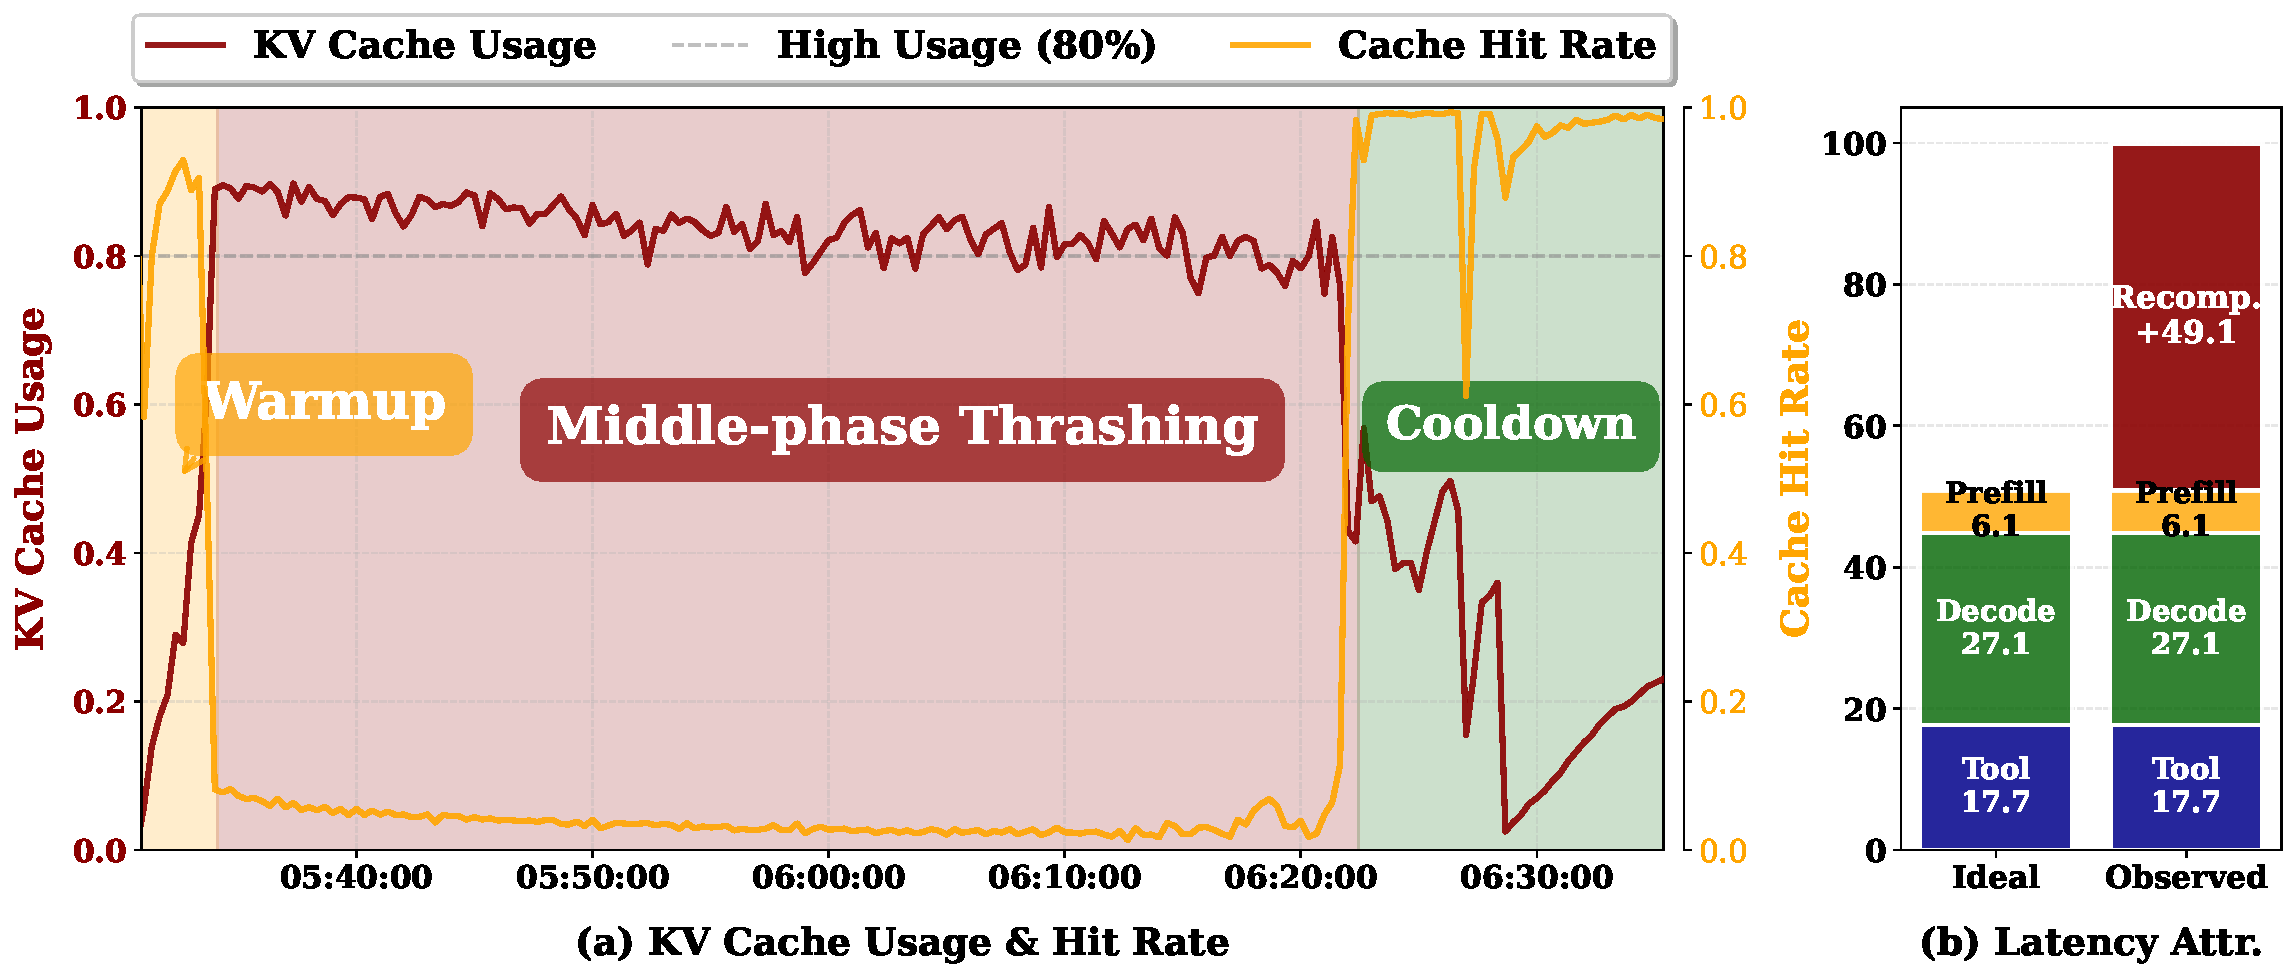
\includegraphics[width=0.98\linewidth]{figure/combined_figure.pdf}

\caption{\textbf{Middle-phase thrashing in real-world agentic batch inference.}
(a) End-to-end KV cache usage over time when running a benchmark on DeepSeek-V3.
The trace exhibits a characteristic three-phase execution pattern in batch agent inference.
(b) End-to-end latency breakdown of the same run, showing the fraction of time spent in prefill and decode, and additional recomputation overhead induced by KV cache thrashing during the middle phase.}
\label{fig:dpskthrashing}
    % \vvspace{}
\end{figure}

\subsection{Characterizing Middle-Phase Thrashing via Empirical Analysis}
\label{subsec:character-middle-phase}
To understand the resource dynamics of agentic batch inference, we analyze execution traces from a large-scale deployment of DeepSeek-V3-based agents under high concurrency. Figure \ref{fig:dpskthrashing} presents the time-series evolution of aggregate GPU KV cache usage and the corresponding cache hit rate. The result reveals that agentic workloads do not exhibit uniform resource consumption regarding aggregate KV cache usage and efficiency. Alternatively, they follow a characteristic three-phase pattern dominated by a phenomenon we term \textbf{Middle-Phase Thrashing}.

(1) \noindent\textbf{Warmup Phase}. During the initial execution stage (yellow shaded area in Figure~\ref{fig:dpskthrashing}), agents operate at shallow reasoning depths with limited context lengths and shared prefixes of prompts. 
Consequently, KV cache footprints remain small and exhibit high similarity, enabling the serving engine to maximize prefix sharing (KV cache hit rates approach 90\%). In this phase, increasing concurrency yields monotonic throughput gains as the aggregate working set remains well within memory constraints.
% As observed in the trace, the system maintains high cache hit rates (approaching 100\%) despite growing concurrency. This efficiency stems from the high degree of prefix sharing (e.g., common system prompts) and small per-agent memory footprints, which allow the aggregate working set to fit comfortably within the GPU memory capacity.
% During this phase, increasing concurrency should yield monotonic throughput gains. GPU utilization scales efficiently as the aggregate working set remains well within memory constraints.

(2) \noindent\textbf{Middle Phase with Thrashing}. 
As agents advance into mid-horizon steps, the system enters the prolonged middle-phase thrashing that dominates over 90\% of the total execution time. 
Figure~\ref{fig:dpskthrashing} illustrates a critical performance pathology and characterizes middle-phase thrashing: while KV cache usage remains consistently near saturation (approx. 80-100\%), the cache hit rate drops precipitously and remains low. The sustained low hit rate indicates the system is trapped in a cycle of eviction and recomputation, rather than being memory-bound in the traditional sense of useful utilization. We observe that this extra recomputation takes 49.1\% of the end-to-end latency compared to other execution stages including prefill, decode, and tool calling in the whole lifecycle. During this phase, increasing concurrency paradoxically degrades overall throughput as it violates the venerable thrashing mitigation~\cite{workingsetmodel}. 


% It is driven by the two characteristics of agentic batch inference mentioned above. 
% As reasoning progresses, agent contexts lengthen and diverge, diminishing opportunities for prefix sharing and eliminating the benefits seen in the warmup phase. The growth of context length also rapidly increases aggregate memory demand. 
% Since agents progress asynchronously and may encounter frequent pausing and resuming due to tool calling, the active working set of KV cache blocks becomes highly volatile. 
% This volatility triggers aggressive eviction once GPU memory usage is high, resulting in frequent preemption of the KV cache across different agents. 
% The system finally enters a regime we term middle-phase thrashing, characterized by saturated KV cache usage simultaneous with collapsing cache hit rates. 
% Meanwhile, agents alternate between generation and tool execution asynchronously, leaving the active working set of KV cache blocks highly volatile. 
% This volatility exacerbates aggressive eviction once GPU memory usage is high, resulting in frequent preemption and expensive prefill recomputation of the KV cache across different agents.


(3) \noindent\textbf{Cooldown Phase}. 
Eventually, as a subset of agents complete their workflows and release memory, the aggregate pressure subsides. The frequency of evictions decreases, allowing the cache hit rate to partially recover as the system exits the thrashing regime.


These observations demonstrate that the primary bottleneck in high-throughput agentic serving is not the peak memory capacity itself, but the reactive nature of existing memory management during the volatile middle phase.

\subsection{Implications for System Design}
% The above analysis highlights a fundamental limitation of existing LLM serving engines.
% Current controllers and memory managers operate at the granularity of individual LLM requests.
% They lack visibility into agent-level progress and are therefore unable to distinguish between temporarily inactive agents and completed or low-priority ones.
% As a result, eviction and scheduling decisions are reactive and myopic, amplifying thrashing rather than stabilizing them.
% Mitigating middle-phase thrashing requires proactive regulation of concurrency based on agent-level state, rather than reactive eviction at the token or request level.
% This insight motivates the design presented in the next section.
% We introduce a controller positioned between the agent execution framework and the LLM serving engine, which treats each agent as a first-class scheduling unit.
% By combining agent-level admission control with adaptive concurrency regulation inspired by AIMD, our system prevents overcommitment of KV cache capacity and maintains stable, high-throughput execution throughout the agent lifecycle.

The prevalence of middle-phase thrashing highlights a fundamental abstraction mismatch in current LLM serving stacks. 
Existing serving engines utilize request-level scheduling, treating each generation step as an isolated, stateless unit of work. 
While effective for standard chat completion, this stateless abstraction fails to capture the long-term state continuity inherent in agentic workflows. 

To address this, we argue that the system design must undergo a paradigm shift along two dimensions: from request-level to agent-level scheduling granularity, and from reactive eviction to proactive admission. 
These two principles motivate the design of \SysName, as detailed below. 


